\documentclass{report}

%                       MAIN PACKAGES                       %
% --------------------------------------------------------- %

\usepackage[english]{babel}
\usepackage{graphicx}
\usepackage{caption}
\usepackage{isolatin1}
\usepackage{amssymb}
\usepackage{textcomp}
\usepackage[usenames,dvipsnames]{color}
\usepackage{soul}
\usepackage{cancel}
\usepackage{booktabs}
\usepackage{multirow}
\usepackage{framed}
\usepackage[table]{xcolor}
\usepackage{algpseudocode}
\usepackage[linesnumbered]{algorithm2e} % for psuedo code
\usepackage{courier}
\usepackage{mathtools} % loads amsmath
\usepackage{forest}
\usepackage{tikz}
\usepackage{tikz-qtree}
\usepackage{interval}
\usetikzlibrary{positioning}
\usetikzlibrary{calc}

%                         MARGINS                           %
% --------------------------------------------------------- %

\hoffset=-0.5in
\voffset=-0.6in
\oddsidemargin=0pt
\topmargin=0pt
\headheight=12pt
\headsep=15pt
\textheight=690pt
\textwidth=543pt
\marginparsep=11pt
\marginparwidth=54pt
\footskip=25pt
\marginparpush=5pt
\paperwidth=597pt
\paperheight=845pt

%                        PAGE STYLE                         %
% --------------------------------------------------------- %

\usepackage{fancyhdr}
\pagestyle{fancy}
\lhead{CLRS {--} Chapter 8 {--} Sorting in Linear Time}
\rhead{Daniel Bastos Moraes}
\cfoot{}
\rfoot{\thepage}
\renewcommand{\headrulewidth}{0.4pt}
\renewcommand{\footrulewidth}{0.4pt}
\newcommand{\Perp}{\perp\! \! \! \perp}


%                       DEFINITIONS                         %
% --------------------------------------------------------- %

\setlength{\parindent}{0cm}

\makeatletter
\renewenvironment{framed}{%
 \def\FrameCommand##1{\hskip\@totalleftmargin
 \fboxsep=\FrameSep\fbox{##1}}%
 \MakeFramed {\advance\hsize-\width
   \@totalleftmargin\z@ \linewidth\hsize
   \@setminipage}}%
 {\par\unskip\endMakeFramed}
\makeatother

\makeatletter
\def\BState{\State\hskip-\ALG@thistlm}
\makeatother

\DeclarePairedDelimiter{\ceil}{\lceil}{\rceil}
\DeclarePairedDelimiter{\floor}{\lfloor}{\rfloor}
\DeclareMathOperator{\Exists}{\exists}
\DeclareMathOperator{\Forall}{\forall}

\def\figuredirectory{images}

\mathchardef\mhyphen="2D % Define a "math hyphen"

\tikzset{every tree node/.style={minimum width=1.95em,draw,circle,font=\footnotesize},
         blank/.style={draw=none},
         edge from parent/.style=
         {draw, edge from parent path={(\tikzparentnode) -- (\tikzchildnode)}},
         level distance=1cm}

\DeclareMathOperator{\di}{d\!}
\newcommand*\Eval[3]{\left.#1\right\rvert_{#2}^{#3}}

\intervalconfig{soft open fences}

\let\oldnl\nl% Store \nl in \oldnl
\newcommand{\nonl}{\renewcommand{\nl}{\let\nl\oldnl}}% Remove line number for one line

\tikzset{
node of list/.style = {
             draw,
             fill=orange!20,
             minimum height=4.5mm,
             minimum width=4.5mm,
             node distance=6mm
   },
link/.style = {
     -stealth,
     shorten >=1pt
     },
array element/.style = {
    draw, fill=white,
    minimum width = 7mm,
    minimum height = 5mm
  }
}

\def\LinkedList#1{%
  \foreach \index/\element in \list {
     \node[node of list, right = of aux, name=\index] {\element};
     \node[node of list, name=aux2, anchor=west] at ([xshift=-.4pt] \index.east) {};
     \draw[link] (aux) -- (\index);
     \coordinate (aux) at (aux2);
   }
   \fill (aux) circle(2pt);
}

%                        DOCUMENT                           %
% --------------------------------------------------------- %

\begin{document}

\small

{\large Section 8.1 {--} Lower bounds for sorting}

\begin{enumerate}

\item[8.1{-}1]{What is the smallest possible depth of a leaf in a decision tree
for a comparison sort?}

\begin{framed}
The smallest possible depth of a leaf in a decision tree
can be obtained by calculating the shortest simple path from the root to any
of its reachable leaves. This smallest path occurs when the comparisons is made
in the sorted order. For instance, if the input array is sorted, the following
comparisons suffices
\begin{equation*}
\begin{aligned}
  a_1 &\le a_2,\\
  a_2 &\le a_3,\\
  &\;\;\vdots\\
  a_{n - 1} &\le a{n}.
\end{aligned}
\end{equation*}

Thus, the smallest depth of a leaf is any decision tree is $n - 1 = \Theta(n)$.

\end{framed}

\item[8.1{-}2]{Obtain asymptotically tight bounds on $\lg(n!)$ without using
Stirling's approximation. Instead, evaluate the summation $\sum_{k = 1}^n \lg k$
using techniques from Section A.2.}

\begin{framed}
Assume for convenience that $n$ is even. For a lower bound, we have
\begin{equation*}
\begin{aligned}
  \lg{n!} &=   \lg(n \cdot (n - 1) \cdot (n - 2) \cdots 1)\\
          &=   \sum_{k = 1}^{n} \lg k\\
          &=   \sum_{k = 1}^{n/2} \lg k + \sum_{k = n/2 + 1}^{n} \lg k\\
          &\ge \sum_{k = 1}^{n/2} 0 + \sum_{k = n/2 + 1}^{n} \lg (n/2)\\
          &=   \frac{n}{2} \lg{\frac{n}{2}}\\
          &=   \frac{n}{2} \lg n - \frac{n}{2}\\
          &=   \Omega(n \lg n).
\end{aligned}
\end{equation*}

And for an upper bound, we have
\begin{equation*}
\begin{aligned}
  \lg{n!} &=   \lg(n \cdot (n - 1) \cdot (n - 2) \cdots 1)\\
          &=   \sum_{k = 1}^{n} \lg k\\
          &\le \sum_{k = 1}^{n} \lg n\\
          &=   O(n \lg n).
\end{aligned}
\end{equation*}

Thus, $\lg n! = \Theta(n \lg n)$.
\end{framed}

\newpage

\item[8.1{-}3]{Show that there is no comparison sort whose running time is
linear for at least half of the $n!$ inputs of length $n$. What about a fraction
of $1/n$ of the inputs of length $n$?  What about a fraction $1/2^n$?}

\begin{framed}
Such algorithm only exists if we can build a decision tree such that at least
$n!/2$ of its $n!$ leaves has a depth of $\Theta(n)$. Suppose this decision tree
exists. Let $m$ be the depth of the leaf with the ($n!/2$)th smallest depth.
Remove all nodes with depth greater than $m$. The result is a decision tree
with height $m$ and at least $n!/2$ leaves. Using the same reasoning as in the
proof of Theorem 8.1, for every decision tree with at least $n!/2$ leaves, we
have
\[
  \frac{n!}{2} \le l \le 2^{m},
\]
which implies
\[
  m \ge \lg \frac{n!}{2} = \lg n! - 1 = \Omega(n \lg n),
\]
which proves that such a decision tree does not exists. The same reasoning can
be applied to obtain the maximum depth of any fraction of the inputs. For
a fraction of $1/n$, we have
\[
  m \ge \lg \frac{n!}{n} = \lg n! - \lg n = \Omega(n \lg n),
\]
and for a fraction of $1/2^n$, we have
\[
  m \ge \lg \frac{n!}{2^n} = \lg n! - \lg 2^n = \lg n! - n = \Omega(n \lg n).
\]
\end{framed}

\item[8.1{-}4]{Suppose that you are given a sequence of $n$ elements to sort.
The input sequence consists of $n/k$ subsequences, each containing $k$ elements.
The elements in a given subsequence are all smaller than the elements in the
succeeding subsequence and larger than the elements in the preceding
subsequence. Thus, all that is needed to sort the whole sequence of length
$n$ is to sort the $k$ elements in each of the $n/k$ subsequences. Show an
$\Omega(n \lg k)$ lower bound on the number of comparisons needed to solve this
variant of the sorting problem. (\emph{Hint}: It is not rigorous to simply
combine the lower bounds for the individual subsequences.)}

\begin{framed}
All we know is the ordering of the elements of a given subsequence with respect
to the elements of the previous/next subsequence. Thus, for each subsequence,
we have $k!$ possible permutations. Since there are $n/k$ input subsequences,
the number of possible outcomes for this sorting problem is
\[
  \prod_{i = 1}^{n/k} k! = k!^{(n/k)}.
\]

We can use here the same argument used in the text book to prove a lower bound
for any comparison sort algorithm. However, in this case, the number of possible
permutations is $k!^{(n/k)}$, instead of $n!$.  Thus, we need to show that the
height of any decision tree with at least $k!^{(n/k)}$ leaves is
$\Omega(n \lg k)$.  We have
\[
  k!^{n/k} \le l \le 2^h,
\]
which implies
\begin{equation*}
\begin{aligned}
h &\ge \lg \left( k!^{(n/k)} \right)\\
  &=   \frac{n}{k} \cdot \lg k!\\
  &=   \frac{n}{k} \cdot \sum_{i = 1}^{k} \lg i\\
  &=   \frac{n}{k} \cdot \sum_{i = 1}^{\floor{k/2}} \lg i + \frac{n}{k} \cdot \sum_{i = \floor{k/2} + 1}^{k} \lg i\\
  &\ge \frac{n}{k} \cdot \sum_{i = \floor{k/2}}^{k} \lg i\\
  &\ge \frac{n}{k} \cdot \left( \frac{k}{2} \lg \frac{k}{2} \right)\\
  &=   \frac{n}{2} \lg \frac{k}{2}\\
  &=   \Omega(n \lg k).\\
\end{aligned}
\end{equation*}
\end{framed}

\end{enumerate}

\newpage

{\large Section 8.2 {--} Counting sort}

\begin{enumerate}

\item[8.2-1]{Using Figure 8.2 as a model, illustrate the operation of
\textsc{Counting-Sort} on the array
$A = \langle 6, 0, 2, 0, 1, 3, 4, 6, 1, 3, 2 \rangle$.}

\begin{framed}
\newcommand\x{${--}$}
\newcommand\y{\cellcolor{white}}
\newcommand\z{\rowcolor{gray!15}}
\[
\begin{array}{cccccccccccc c cccccccc}
  \y   & 1  & 2  & 3  & 4  & 5  & 6  & 7  & 8  & 9  & 10 & 11 & \y &
  \y   & 0  & 1  & 2  & 3  & 4  & 5  & 6\\
  \z
  \y A & 6  & 0  & 2  & 0  & 1  & 3  & 4  & 6  & 1  & 3  & 2  & \y &
  \y C & 2  & 2  & 2  & 2  & 1  & 0  & 2\\\\
  \z
  \y   & \y & \y & \y & \y & \y & \y & \y & \y & \y & \y & \y & \y &
  \y C & 2  & 4  & 6  & 8  & 9  & 9  & 11\\\\
  \z
  \y B & \x & \x & \x & \x & \x & 2  & \x & \x & \x & \x & \x & \y &
  \y C & 2  & 4  & 5  & 8  & 9  & 9  & 11\\\\
  \z
  \y B & \x & \x & \x & \x & \x & 2  & \x & 3  & \x & \x & \x & \y &
  \y C & 2  & 4  & 5  & 7  & 9  & 9  & 11\\\\
  \z
  \y B & \x & \x & \x &  1 & \x & 2  & \x & 3  & \x & \x & \x & \y &
  \y C & 2  & 3  & 5  & 7  & 9  & 9  & 11\\\\
  \z
  \y B & \x & \x & \x &  1 & \x & 2  & \x & 3  & 4  & \x & 6  & \y &
  \y C & 2  & 3  & 5  & 7  & 8  & 9  & 10\\\\
  \z
  \y B & \x & \x & \x &  1 & \x & 2  & 3  & 3  & 4  & \x & 6  & \y &
  \y C & 2  & 3  & 5  & 6  & 8  & 9  & 10\\\\
  \z
  \y B & \x & \x & 1  &  1 & \x & 2  & 3  & 3  & 4  & \x & 6  & \y &
  \y C & 2  & 2  & 5  & 6  & 8  & 9  & 10\\\\
  \z
  \y B & \x & 0  & 1  &  1 & \x & 2  & 3  & 3  & 4  & \x & 6  & \y &
  \y C & 1  & 2  & 5  & 6  & 8  & 9  & 10\\\\
  \z
  \y B & \x & 0  & 1  &  1 & 2  & 2  & 3  & 3  & 4  & \x & 6  & \y &
  \y C & 1  & 2  & 4  & 6  & 8  & 9  & 10\\\\
  \z
  \y B & 0  & 0  & 1  &  1 & 2  & 2  & 3  & 3  & 4  & \x & 6  & \y &
  \y C & 0  & 2  & 4  & 6  & 8  & 9  & 10\\\\
  \z
  \y B & 0  & 0  & 1  &  1 & 2  & 2  & 3  & 3  & 4  & 6  & 6  & \y &
  \y C & 0  & 2  & 4  & 6  & 8  & 9  & 9
\end{array}
\]
\end{framed}

\item[8.2-2]{Prove that \textsc{Counting-Sort} is stable.}

\begin{framed}
Suppose that the integer $x$ appears $k$ times in the output array. Since the
\textbf{for} loop of lines 10-12 iterates over the input array backwards, the
first integer $x$ to be added to the output array on line 11 is the rightmost
one. The decrement of the couting of $x$ on line 12 ensures that the next
integer $x$ is added to the output array right before the previous one. This
process repeats $k$ times, until the leftmost integer $x$ is added to the
output array ($k - 1$ positions before the rightmost one). This property ensures
that elements with equal value in the input array appears in the same order in
the output array. Thus, the algorithm is stable.
\end{framed}

\item[8.2-3]{Suppose that we were to rewrite the \textbf{for} loop header in
line 10 of the \textsc{Counting-Sort} as

$10\quad\text{\textbf{for}}\;j = 1\;\text{\textbf{to}}\;A.length$

Show that the algorithm still works properly. Is the modified algorithm stable?
}

\begin{framed}
The only difference will be in the \textbf{for} loop of lines 10-12, in which
elements with equal value in the input array will now be added to the output
array in the same order as they appear in the input array. As observed on
Question 8.2-2, each time an element with value $x$ is added to the output
array, the next element with value $x$ is added right before the previous one.
This implies that elements with equal value in the input array will appear in
reverse order in the output array. Thus, this modified algorithm is not stable.
\end{framed}

\item[8.2-4]{Describe an algorithm that, given $n$ integers in the range $0$ to
$k$, preprocesses its input and then answers any query about how many of the $n$
integers fall into a range $[a \dots b]$ in $O(1)$ time. Your algorithm should
use $\Theta(n + k)$ preprocessing time.}

\begin{framed}
For the preprocessing phase, build the array $C$ in the same way it is built in
the \textsc{Couting-Sort} procedure (lines 1-8). This preprocessing will run in
$\Theta(k) + \Theta(n) + \Theta(k) = \Theta(n + k)$. If $a > 0$, answer
$C[b] - C[a - 1]$. Otherwise, answer $C[b]$.
\end{framed}

\end{enumerate}

\newpage

{\large Section 8.3 {--} Radix sort}

\begin{enumerate}

\item[8.3-1]{Using Figure 8.3 as a model, illustrate the operation of
\textsc{Radix-Sort} on the following list of English words: COW, DOG, SEA, RUG,
ROW, MOB, BOX, TAB, BAR, EAR, TAR, DIG, BIG, TEA, NOW, FOX.}

\begin{framed}
\newcommand{\x}[1]{\textbf{#1}}
\begin{center}
\texttt{
\begin{tabular}{c}
  COW\\
  DOG\\
  SEA\\
  RUG\\
  ROW\\
  MOB\\
  BOX\\
  TAB\\
  BAR\\
  EAR\\
  TAR\\
  DIG\\
  BIG\\
  TEA\\
  NOW\\
  FOX
\end{tabular}
}
$\rightarrow$
\texttt{
\begin{tabular}{c}
  SE\x{A}\\
  TE\x{A}\\
  MO\x{B}\\
  TA\x{B}\\
  DO\x{G}\\
  RU\x{G}\\
  DI\x{G}\\
  BI\x{G}\\
  BA\x{R}\\
  EA\x{R}\\
  TA\x{R}\\
  CO\x{W}\\
  RO\x{W}\\
  NO\x{W}\\
  BO\x{X}\\
  FO\x{X}
\end{tabular}
}
$\rightarrow$
\texttt{
\begin{tabular}{c}
  T\x{A}B\\
  B\x{A}R\\
  E\x{A}R\\
  T\x{A}R\\
  S\x{E}A\\
  T\x{E}A\\
  D\x{I}G\\
  B\x{I}G\\
  M\x{O}B\\
  D\x{O}G\\
  C\x{O}W\\
  R\x{O}W\\
  N\x{O}W\\
  B\x{O}X\\
  F\x{O}X\\
  R\x{U}G
\end{tabular}
}
$\rightarrow$
\texttt{
\begin{tabular}{c}
  \x{B}AR\\
  \x{B}IG\\
  \x{B}OX\\
  \x{C}OW\\
  \x{D}IG\\
  \x{D}OG\\
  \x{E}AR\\
  \x{F}OX\\
  \x{M}OB\\
  \x{N}OW\\
  \x{R}OW\\
  \x{R}UG\\
  \x{T}AB\\
  \x{T}AR\\
  \x{T}EA\\
  \x{S}EA
\end{tabular}
}
\end{center}
\end{framed}

\item[8.3-2]{Which of the following sorting algorithms are stable: insertion
sort, merge sort, heapsort, and quicksort? Give a simple scheme that makes any
comparison sort stable. How much additional time and space does your scheme
entail?}

\begin{framed}
\textsc{Insertion-Sort} and \textsc{Merge-Sort} are stable. \textsc{Heapsort}
and \textsc{Quicksort} are not. To make any sorting algorithm stable, we can
store the original index of each element in the array and use this index to
break ties. The additional space required is $\Theta(n)$. The asymptotic running
time is the same, since the number of comparisons will be at most twice.
\end{framed}

\item[8.3-3]{Use induction to prove that radix sort works. Where does your proof
need the assumption that the intermediate sort is stable?}

\begin{framed}
Let $d$ be the number of columns in the input array, where the $d$th column
contains the highest-order digit. \textsc{Radix-Sort} sorts one column at
a time, from the column with the lowest-order digits to the column with the
highest-order digits. The base case occurs when $d = 1$. Since in this case the
elements on the array has a single digit, calling \textsc{Radix-Sort} in this
case is the same as calling its sorting subroutine directly with the input array
as an argument. Thus, \textsc{Radix-Sort} is correct when $d = 1$. Now assume
\textsc{Radix-Sort} works for $d - 1$ columns. Note that sorting $d$ columns is
equivalent to sorting $d - 1$ columns followed by calling the sorting subroutine
on the $d$th column. The induction hypothesis ensures that \textsc{Radix-Sort}
sorts $d - 1$ columns correctly. Since the sorting subroutine is stable, when
sorting the $d$th column, digits that have the same value in the $d$th column
will be kept in the same order as it was after sorting the $(d - 1)$th column.
This implies that \textsc{Radix-Sort} breaks ties on higher-order digits by the
lower-order digits, which is correct.

The sorting subroutine must be stable since a tie that occur while sorting the
$i$th digit is determined by the previous sorts of the lower-order digits. Since
lower-order digits are sorted before higher-order digits, this property is
ensured with an stable sorting algorithm.
\end{framed}

\item[8.3-4]{Show how to sort $n$ integers in the range $0$ to $n^3 - 1$ in
$O(n)$ time.}

\begin{framed}
An integer in the range $0$ to $n^3 - 1$ is represented with at most
$\lg n^3 = 3 \lg n$ bits. We can view a $(3 \lg n)$-bit integer as three
$(\lg n)$-bit integers, so that $b = 3 \lg n$ and $r = \lg n$. With these
settings, \textsc{Radix-Sort} correctly sorts these numbers in
\[
  \Theta\left( \frac{b}{r} \left( n + 2^r \right) \right)
  = \Theta\left( \frac{3 \lg n}{\lg n} \left(n + 2^{\lg n}\right) \right)
  = \Theta( 3 (n + n) )
  = \Theta(n).
\]
\end{framed}

\newpage

\item[8.3-5]{($\star$) In the first card-sorting algorithm in this section,
exactly how many sorting passes are needed to sort $d$-digit decimal numbers in
the worst case? How many piles of cards would an operator need to keep track of
in the worst case?}

\begin{framed}
Suppose that the card-sorting machine represents numbers in base $p$, such
that $2 \le p \le 10$. For a given value of $p$, we have
\begin{itemize}
  \item Each card uses $c = \ceil{\log_p 10^d}$ columns;
  \item Each column uses up to $p$ places.
\end{itemize}

Let $c$th-digit denote the most significant digit, the $(c - 1)$th-digit
denote the 2nd most significant digit, and so on.

The algorithm is recursive. It starts sorting on the $c$th-digit, which
requires $p$ piles to distribute the cards in the worst-case. In the next level,
the algorithm sorts each of the $p$ piles on the $(c - 1)$th-digit, which
requires $p^2$ piles to distribute the cards in the worst-case (each of the
$p$ piles is splitted into $p$ piles). This process goes for $c$ levels. Since
the piles of the previous level can be reutilized in the current level, the
number of piles required to distribute the cards in all levels is the number of
piles required in the last level, which is
\[
  p^c.
\]

Note that to sort the cards on the $c$th-digit, only one sorting pass is needed
to distribute the cards into $p$ piles. To sort on the next digit, these $p$
piles that were sorted on the $c$th-digit must now be sorted on the
$(c - 1)$th-digit, which will require another $p^1$ sorting passes to distribute
them into $p^2$ piles. In general, to sort on the $i$th digit, $p^{c - i}$
sorting passes are required in the worst-case. Thus, the number of sorting
passes in the worst-case is
\[
  \sum_{i = 1}^{c} p^{c - i} = \sum_{i = 0}^{c - 1} p^{i} = \frac{p^c - 1}{p - 1}.
\]

\end{framed}

\end{enumerate}

\newpage

{\large Section 8.4 {--} Bucket sort}

\begin{enumerate}

\item[8.4-1]{Using Figure 8.4 as a model, illustrate the operation of
\textsc{Bucket-Sort} on the array
$A = \langle .79, .13, .16, .64, .39, .20, .89, .53, .71, .42 \rangle$.}

\begin{framed}
\begin{center}
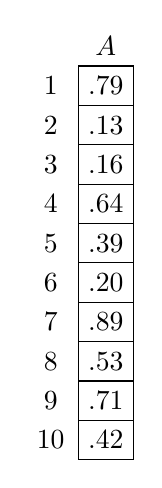
\begin{tikzpicture}
\node at (0, 0) {$A$};
\foreach \index/\element/\list in {1/.79, 2/.13, 3/.16, 4/.64, 5/.39, 6/.20,
                                   7/.89, 8/.53, 9/.71, 10/.42} {
   \node[array element] (aux) at (0,-\index/2) {\element};
   \node at (-0.7, -\index/2) {\index};
}
\end{tikzpicture}
\qquad
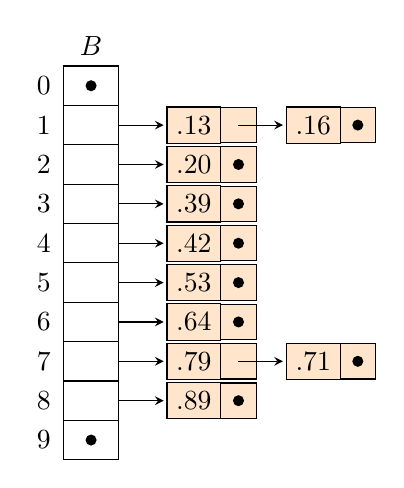
\begin{tikzpicture}
\node at (0, 0.5) {$B$};
  \foreach \index/\list in {0/, 1/{1/.13, 2/.16}, 2/{1/.20}, 3/{1/.39},
                            4/{1/.42}, 5/{1/.53}, 6/{1/.64}, 7/{1/.79, 2/.71},
                            8/{1/.89}, 9/} {
   \node[array element] (aux) at (0,-\index/2) {};
   \node at (-0.6, -\index/2) {\index};
   \LinkedList{\list}
}
\end{tikzpicture}
\end{center}
\end{framed}

\item[8.4-2]{Explain why the worst-case running time for bucket sort is
$\Theta(n^2)$. What simple change to the algorithm preserves its linear
average-case running time and makes its worst-case running time $O(n \lg n)$?}

\begin{framed}
The worst-case occurs when the input array is in decreasing order and every
element falls into the same bucket. Since \textsc{Insertion-Sort} takes
$\Theta(n^2)$ to sort an array of size $n$ that is in decreasing order, bucket
sort will run in $\Theta(n^2)$.

The worst-case running time can be improved replacing \textsc{Insertion-Sort}
with $\textsc{Heapsort}$, which will make it run in $O(n \lg n)$. As for the
average-case, the expected running time of this variation of bucket sort is
\begin{equation*}
\begin{aligned}
  \text{E}[T(n)] &= \text{E}\left[ \Theta(n) + \sum_{i = 0}^{n - 1} O(n_i \lg n_i) \right]\\
                 &= \Theta(n) + \sum_{i = 0}^{n - 1} \text{E}[O(n_i \lg n_i)]\\
                 &= \Theta(n) + \sum_{i = 0}^{n - 1} O(\text{E}[n_i \lg n_i]).
\end{aligned}
\end{equation*}

Using the same logic adopted in the text book to compute $\text{E}[n_i^2]$, we
have
\[
  n_i = \sum_{j = 1}^{n} X_{ij},
\]
which implies
\begin{equation*}
\begin{aligned}
  \text{E}[n_i \lg n_i] &=   \text{E}\left[ \sum_{j = 1}^{n} X_{ij} \lg \sum_{j = 1}^{n} X_{ij} \right]\\
                        &\le \text{E}\left[ \sum_{j = 1}^{n} X_{ij} \sum_{j = 1}^{n} X_{ij} \right]\\
                        &=   2 - \frac{1}{n}. & \text{(from equation (8.2))}
\end{aligned}
\end{equation*}

Thus, the average-case running time of this variation of bucket sort is
\[
  \text{E}[T(n)] = \Theta(n) + \sum_{i = 0}^{n - 1} O\left(2 - \frac{1}{n}\right)
                 = \Theta(n) + n \cdot O\left(1\right)
                 = \Theta(n).
\]
\end{framed}

\newpage

\item[8.4-3]{Let $X$ be a random variable that is equal to the number of heads
in two flips of a fair coin. What is $\text{E}[X^2]$? What is $\text{E}^2[X]$?}

\begin{framed}
Lets define the indicator random variable
\[
  X_i = \text{I}\{\text{flip } i \text{ comes up heap}\}.
\]

Thus, we have
\[
  X = X_1 + X_2,
\]
and
\[
  X^2 = (X_1 + X_2)^2 = X_1^2 + 2 X_1 X_2 + X_2^2.
\]

Note that
\[
  \text{E}[X_i] = \text{Pr}\{X_i = 1\} = \frac{1}{2},
\]
and
\[
  \text{E}[X_i^2] = 1^2 \cdot \frac{1}{2} + 0^2 \cdot \frac{1}{2} = \frac{1}{2}.
\]

Using the above definitions and linearity of expectation, we have
\begin{equation*}
\begin{aligned}
  \text{E}[X^2] &= \text{E}[X_1^2 + 2 X_1 X_2 + X_2^2]\\
                &= \text{E}[X_1^2] + 2 \text{E}[X_1 X_2] + \text{E}[X_2^2]\\
                &= \frac{1}{2} + 2 \left(\text{E}[X_1] \text{E}[X_2]\right) + \frac{1}{2} & \text{(since $X_1$ and $X_2$ are independent)}\\
                &= \frac{1}{2} + 2 \left(\frac{1}{2} \cdot \frac{1}{2}\right) + \frac{1}{2}\\
                &= \frac{3}{2},
\end{aligned}
\end{equation*}
and
\begin{equation*}
\begin{aligned}
  \text{E}^2[X] &= \text{E}^2[X_1 + X_2]\\
                &= \text{E}[X_1 + X_2] \text{E}[X_1 + X_2]\\
                &= ( \text{E}[X_1] + \text{E}[X_2] ) ( \text{E}[X_1] + \text{E}[X_2] )\\
                &= \left( \frac{1}{2} + \frac{1}{2} \right) \left( \frac{1}{2} + \frac{1}{2} \right)\\
                &= 1.
\end{aligned}
\end{equation*}
\end{framed}

\newpage

\item[8.4-4]{($\star$) We are given $n$ points in the unit circle,
$p_i = (x_i, y_i)$, such that $0 < x^2_i + y^2_i \le 1$ for
$i = 1, 2, \dots, n$. Suppose that the points are uniformly distributed; that
is, the probability of finding a point in any region of the circle is
proportional to the area of that region. Design an algorithm with an
average-case running time of $\Theta(n)$ to sort the $n$ points by their
distances $d_i = \sqrt{x^2_i + y^2_i}$ from the origin. (\emph{Hint:} Design the
bucket sizes in \textsc{Bucket-Sort} to reflect the uniform distribution of the
points in the unit circle.)}

\begin{framed}

Considering that the points are uniformly distributed over the area of the unit
circle, we can divide the circle into $n$ rings with equal area, such that the
expected number of points in each ring is $1$. The figure below illustrates
a circle that is divided into three rings with equal area.

\begin{center}
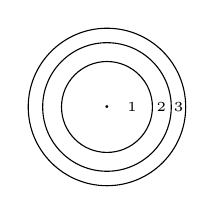
\begin{tikzpicture}[black]
  \draw node at (0.0, 0.0) {.};
  \draw node at (0.32, 0.0) {\tiny 1};
  \draw node at (0.69, 0.0) {\tiny 2};
  \draw node at (0.91, 0.0) {\tiny 3};
  \foreach \i in {1, 2, 3} {
    \draw (0,0) circle ({sqrt(\i) / sqrt(3)});
  }
\end{tikzpicture}
\end{center}

We them assign to the $i$th bucket the points that falls within the $i$th ring,
sort each bucket individually with \textsc{Insertion-Sort}, and combine the
elements of each bucket sequentially. This is basically the \textsc{Bucket-Sort}
algorithm with a modification on the way we assign the elements to the buckets.
Since the distribution of points over the buckets is uniform, the average-case
running time of this algorithm is still $O(n)$.

We now need a function that maps a point to its bucket. Let $r_i$ denote the
(larger) radius of the $i$th ring. We claim that
\[
  r_i = \frac{\sqrt{i}}{\sqrt{n}},
\]
which implies that a point $p_j$ belongs to the $i$th ring if, and only if,
\[
  \sqrt{\frac{i - 1}{n}} < d_j \le \sqrt{\frac{i}{n}},
\]
squaring both sides and multiplying by $n$, we have
\[
  i - 1 < d_j^2 \cdot n \le i
\]
which implies
\[
  i = \ceil{d_j^2 \cdot n}.
\]

\textbf{Proof for the radius of the $i$th ring.}

Since the area of the unit circle is $\pi$ and each ring has equal area, for
$i > 0$, we have
\[
  \pi r_i^2 - \pi r_{i - 1}^2 = \frac{\pi}{n},
\]
which implies
\[
  r_i = \sqrt{\frac{1}{n} + r^2_{i - 1}}.
\]

Note that
\begin{equation*}
\begin{aligned}
  r_1 = \sqrt{\frac{1}{n} + 0^2} = \frac{\sqrt{1}}{\sqrt{n}},\\
  r_2 = \sqrt{\frac{1}{n} + \left(\sqrt{\frac{1}{n}}\right)^2} = \frac{\sqrt{2}}{\sqrt{n}},\\
  r_3 = \sqrt{\frac{1}{n} + \left(\sqrt{\frac{2}{n}}\right)^2} = \frac{\sqrt{3}}{\sqrt{n}},
\end{aligned}
\end{equation*}

which lead us to assume that
\[
  r_i = \frac{\sqrt{i}}{\sqrt{n}},
\]
for $i = 0, 1, \dots, n$. We shall prove it by induction. Note that it holds for
$i = 0$, since
\[
  r_0 = \frac{\sqrt{0}}{\sqrt{n}} = 0.
\]
To show that it holds for $i > 0$, we need to show that if it holds for $i$, it
also holds for $i + 1$. We have
\[
  r_{i + 1} = \sqrt{\frac{1}{n} + \left(\sqrt{\frac{i}{n}}\right)^2}
            = \sqrt{\frac{i + 1}{n}}
            = \frac{\sqrt{i + 1}}{\sqrt{n}},
\]
which proves the inductive step.

\end{framed}

\item[8.4-5]{($\star$) A \textbf{\emph{probability distribution function}}
$P(x)$ for a random variable $X$ is defined by $P(x) = \text{Pr}\{X \le x\}$.
Suppose that we draw a list of $n$ random variables $X_1, X_2, \dots, X_n$ from
a continuous probability distribution function $P$ that is computable in $O(1)$
time. Give an algorithm that sorts these numbers in linear average-case time.}

\begin{framed}
Skipped.
\end{framed}

\end{enumerate}

\end{document}
